% 2010 年广东卷理科第 14 题：圆 O 的两条弦 AB、CD。
% 来源 PDF：普通高考/2010/2010广东理.pdf，SHA-256 1c708f5a82d57782cd31357148f1dba05af44c63ffab0045cf301c88eb5d5fd7。
% 原页：第 1 页（A3 三栏）第 2 栏下部，书页码 593。
% 重绘依据：AB 为圆 O 的弦，P 为 AB 中点，CD 过 P；PD=2a/3，∠OAP=30°。
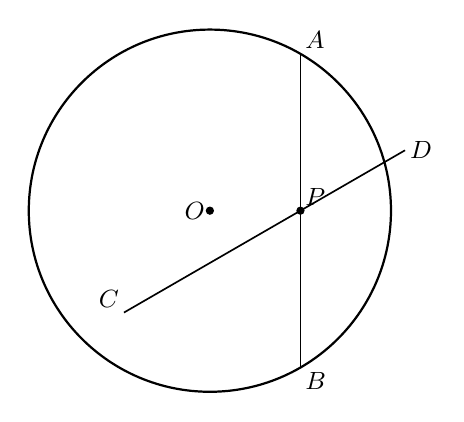
\begin{tikzpicture}[semithick, scale=1.15, every node/.style={inner sep=1.5pt, font=\small}]
  \draw[thick] (0,0) circle (2);
  \coordinate (O) at (0,0);
  \coordinate (P) at (1,0);
  \coordinate (A) at (1,1.732);
  \coordinate (B) at (1,-1.732);
  \coordinate (D) at (2.155,0.667);
  \coordinate (C) at (-0.949,-1.125);
  \draw (A) -- (B);
  \draw (C) -- (D);
  \fill (P) circle (1.3pt);
  \fill (O) circle (1.3pt);
  \node[left] at (O) {$O$};
  \node[above right] at (A) {$A$};
  \node[below right] at (B) {$B$};
  \node[above left] at (C) {$C$};
  \node[right] at (D) {$D$};
  \node[above right] at (P) {$P$};
\end{tikzpicture}
